\documentclass[a4paper, titlepage]{jsarticle}

\date{\today}
\usepackage[dvipdfmx]{graphicx}
\usepackage{url}
\usepackage[T1]{fontenc}
\usepackage{float}
\usepackage{ascmac}
\usepackage{pdfpages}

\title{ドローン宅配事業者支援システム}

\author{土佐山田IT株式会社}

\begin{document}
\maketitle

\tableofcontents

\clearpage

\section{現状の課題}
2022年日本における宅配便取扱個数は50億個を超えた。
\begin{figure}[H]
    \centering
    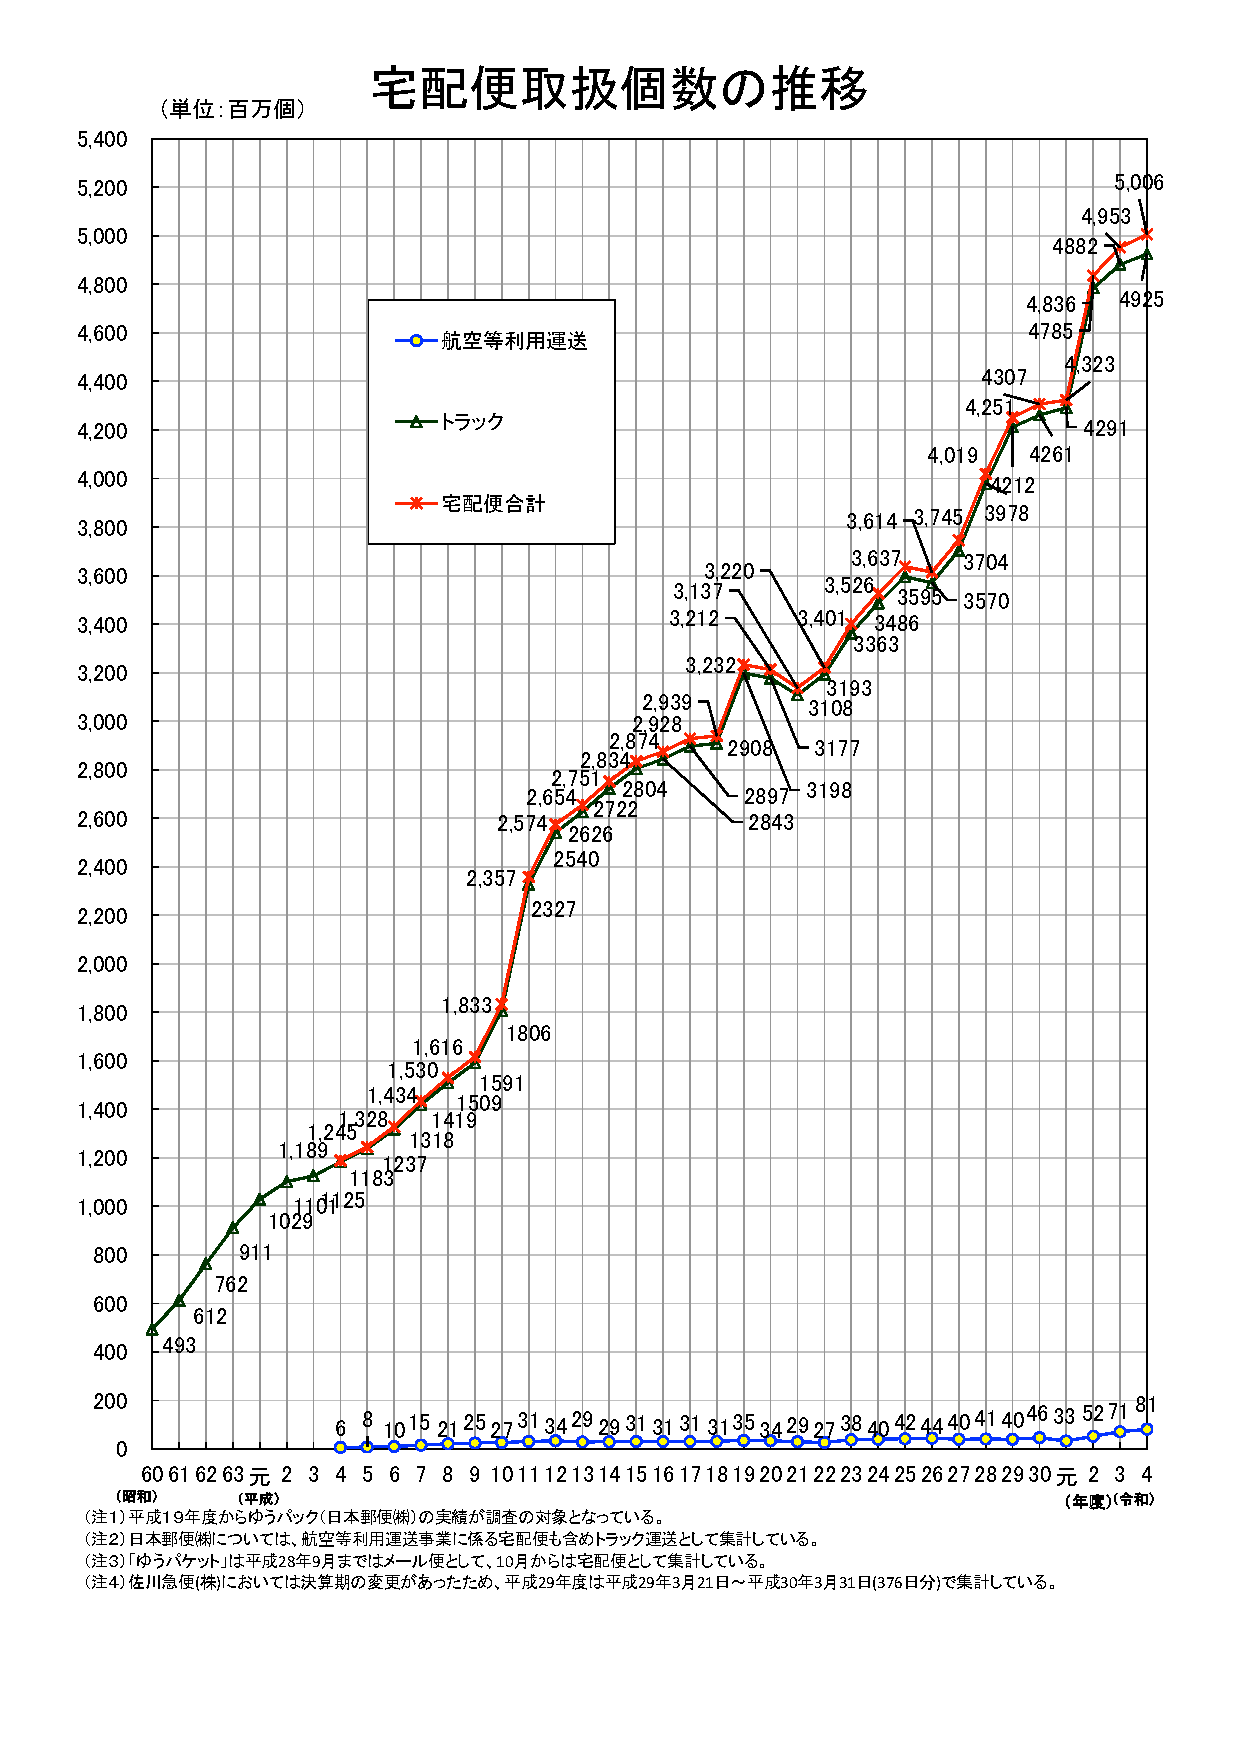
\includegraphics[width=0.6\textwidth]{./home_delivery.pdf}
    \caption{ドローン宅配}
    \label{fig:delivery}
\end{figure}
毎年増加が続いている数字からも分かるように、
現代社会において宅配サービスは日常生活に深く根付いている、しかし宅配需要の増加と少子高齢化社会に伴う労働人口の減少により、現状の宅配サービスを維持することは日々困難になっている。
\begin{figure}[H]
    \centering
    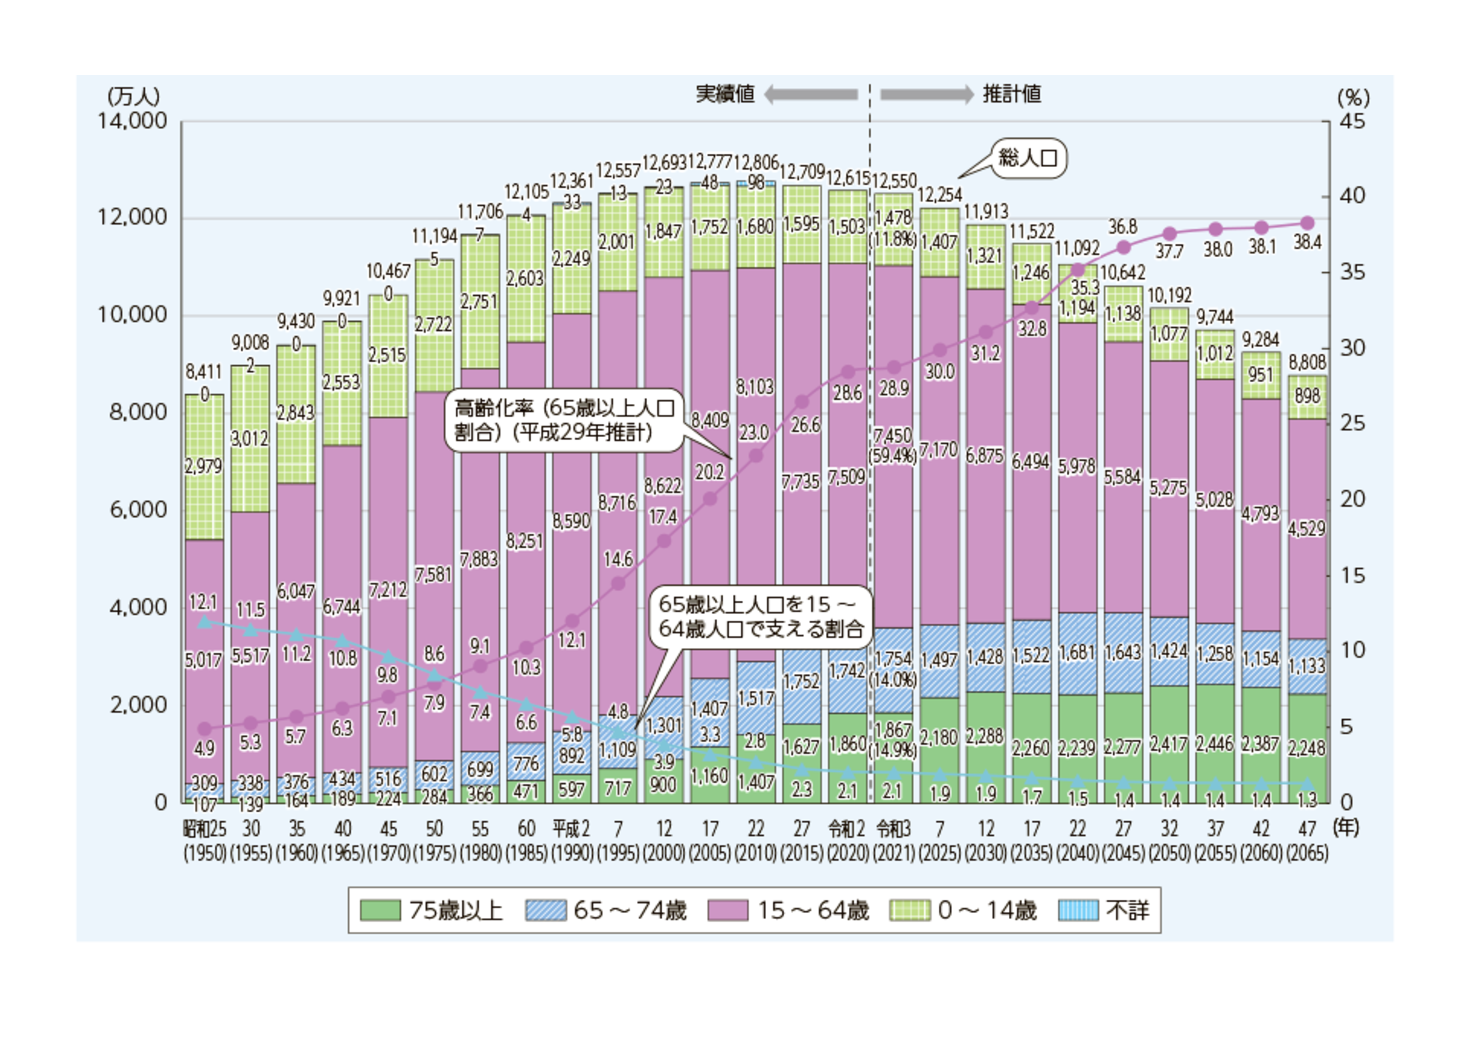
\includegraphics[width=0.8\textwidth]{./working_population.pdf}
    \caption{ドローン宅配}
    \label{fig:delivery}
\end{figure}
特に過疎地域等においては、現状の輸送方法では効率が悪く輸送方法の効率化が求められている。

\section{課題の解決方法}
上記の課題を解決するため、効率的かつ人手不足を解消できるようなドローン宅配宅配事業者支援システムを提案する。
このシステムによる課題の解決方法を以下に示す。
\begin{itemize}
    \item ドローンの操縦を自動化することでより少ない人手で大量の荷物を個人宅に運搬できるようにする。
    \item 宅配事業者の支援システムを多くの事業者に提供することで、より多くの事業者に参入してもらい、競争が生まれることでドローン宅配事業の効率化を進めることができる。
    \item 多くの事業者に共通のシステムを使ってもらうことで、スケールメリットを活かしてコスト削減を進めることが出来る。
    \item 離島や里山の陸路では宅配が大変な地域にも簡単に配送を行うことができる。
\end{itemize}

\section{機能の概要・前提条件・制約事項}
\subsection{機能概要}
本システムは管理者,ドローン宅配事業者,使用者が存在する.それぞれに向けた機能の概要を説明する.
\subsubsection{管理者向け機能}
\begin{itemize}
    \item ログインログアウト機能
    \item 会員管理機能
    \item ドローン宅配事業者会員登録承認機能
    \item 会員情報閲覧機能
    \item 利用情報分析機能
    \item 宅配依頼受付機能
    \item 宅配仕事割り振り機能
    % \item ドローン貸出機能
    % \item 貸出ドローン情報管理機能
\end{itemize}
\subsubsection{ドローン宅配事業者向け機能}
\begin{itemize}
    \item ログインログアウト機能
    \item ドローン宅配事業者会員登録申請
    \item 宅配依頼承諾機能
    \item 配達完了通知機能
    \item 宅配場所登録機能
    %\item ドローンレンタル機能
    \item 退会機能
\end{itemize}
\subsubsection{使用者向け機能}
\begin{itemize}
    \item ログインログアウト機能
    \item 使用者会員登録機能
    \item 宅配依頼機能
    \item 宅配場所登録機能
    \item 退会機能
\end{itemize}
\section{情報・金銭の流れ}

\section{想定する利用者}

\section{運用・保守}

\section{ハードウェア・ソフトウェアの構成}

\section{費用・効果}

\section{スケジュール}

\section{本システムのアピールポイント}

\section{貢献度}


\end{document}
